\documentclass[11pt]{article} % DOKUMENTKLASSE. Mulighederne inkl. article, report, book, memoir  %
                              % Geometri-pakke: Styrer bl.a. maginer                              %
\usepackage[a4paper, hmargin={2.8cm, 2.8cm}, vmargin={2.8cm, 2.8cm}]{geometry}                    %
\usepackage{amssymb}          % Matematiske tegn og skrifttyper, bl.a. \mathbb{}                  %
\usepackage{amsthm}           % Opsætning der gør sætninger og beviser nemmere, se amsthdoc.pdf   %
\usepackage[utf8]{inputenc}   % Lidt kodning så der ikke kommer problemer ved visse konverteringer%
\usepackage[T1]{fontenc}      % Lidt kodning så der ikke kommer problemer ved visse konverteringer%
\usepackage{amsmath}          % Matematiske tegn                                                  %
\usepackage[colorlinks=true]{hyperref}   % Referencer som hyperlinks                              %
%\usepackage{txfonts}         % Times font                                                        %
\usepackage{graphicx}         % Graphicx pakke                                                    %
\usepackage{bigfoot}          % \verb in footnote                                                    %
\usepackage{caption}          % Caption-pakke                                                     %
\usepackage{subcaption}       % Subcaption-pakke                                                  %
\setlength{\captionmargin}{20pt}% Sætter caption-margin                                           %
\usepackage{listings}         % Listings. Indsætter kildekode pænt.                               %
\usepackage{float}            % Keeping figures in place                                          %
\lstset{                      %                                                                   %
  basicstyle=\ttfamily\footnotesize, % Sætter basisstilen i listings                              %
  showstringspaces=false,     % no special string spaces                                          %
  extendedchars=true,         % Bogstaver som æ, ø og å 
}                             %                                                                   %

\usepackage{courier}          % Courierskrifttype. Slankere skrivemaskineskrift i verbatim og     %
                              % listings                                                          %
\usepackage{multicol}         % Kolonner                                                          %
\usepackage[babel, titelside, nat, farve, en]{ku-forside}   % KU-forside med logoer               %
\def\HyperLinks{              % Hyperlinks-pakke, referencer til links og tillader links til www  %
\usepackage[pdftitle={\TITEL},pdfauthor={\FORFATTER}, % Et lille trick så pakken indlæses efter   %
pdfsubject={\UNDERTITEL}, linkbordercolor={0.8 0.8 0.8}]{}} %  titlen defineres.          %
\DeclareSymbolFont{rsfscript}{OMS}{rsfs}{m}{n} % Henter alfabet                                   %
\DeclareSymbolFontAlphabet{\mcal}{rsfscript} % Kalder dette alfabet for \mcal                     %
\setlength\arraycolsep{2 pt}  % Sætter kolonneafstanden i tabeller og eqnarrays til 2pt           %
\setcounter{tocdepth}{3}      % Dybde af indholdsfortegnelsen,                                    %
                              % 1 resulterer i kun sections kommer med, 2 er secs og subsec. etc  %
% \setcounter{secnumdepth}{0}   % Dybde af sektionsnummereringen.                                   %
%%%%%%%%%%%%%%%%%%%%%%%%%%%%%%%%%%%%%%%%%%%%%%%%%%%%%%%%%%%%%%%%%%%%%%%%%%%%%%%%%%%%%%%%%%%%%%%%%%%
\titel{Evaluating scalability of hash-based multi-core in-memory key-value stores} %                 %
\undertitel{Faculty of Computer Science} %                                                        %
\opgave{Thesis Report}                   % Findes kun under 'titelside' muligheden i ku-forside   %
\forfatter{Jakob Hanehoj}                %                                                        %
\dato{\today}                            %                                                        %
\vejleder{Marcos Antonio Vaz Salles and Vivek Shah} % Findes kun under 'titelside' muligheden i KU-forside   %
\HyperLinks                              % Sætter pdf-titel til at svare til de just definerede   %
                                         %                                                        %
\begin{document}                         %                                                        %
\maketitle % Laver titlen                %                                                        %
                                         %                                                        %
%%%%%%%%%%%%%%%%%%%%%%%%%%%%%%%%%%%% Indholdsfortegnelse %%%%%%%%%%%%%%%%%%%%%%%%%%%%%%%%%%%%%%%%%%

\begin{abstract}
\end{abstract}
\tableofcontents % indholdsfortegnelsen                                                           %
\listoffigures  % Liste over figurer \begin{figure} ... \end{figure}                              %
\listoftables   % Liste over tabeller \begin{table} ... \end{table}                               %
%%%%%%%%%%%%%%%%%%%%%%%%%%%%%%%%%%%%%%%%%%%%%%%%%%%%%%%%%%%%%%%%%%%%%%%%%%%%%%%%%%%%%%%%%%%%%%%%%%%

\newpage
\section{Introduction}

\newpage
\section{Background}
\subsection{Key-value stores}
\paragraph{General background, APIs, systems.}
\paragraph{Multi-core implementations.}
\subsection{Hashing algorithms}
\paragraph{Review of hashing algorithms.}
Recently, a thorough comparison of hashing methods has been performed by Richter et al.~\cite{RAD15}, in which they evaluate four hash functions, namely
\begin{itemize}
\item Multiply-shift hashing
\item Multiply-add-shift hashing
\item Murmur hashing
\item Tabulation hashing
\end{itemize}
Since multiply-shift hashing and multiply-add-shift hashing only have implementations for fixed-length keys, we have chosen to focus on murmur hashing and tabulation hashing. They conclude that both of these hashing methods are slower than both multiply-shift hashing and multiply-add-shift hashing, even though both have greater robustness in terms of distributional properties, when faced with skewed input distributions. Between murmur hashing and tabulation hashing, they conclude murmur hashing to be the faster, with tabulation hashing being the most robust. \\
\\
The tabulation hashing algorithm is by no means a new form of hashing, as the first instances of tabulation hashing was published in 1970 by Albert Zobrist~\cite{Zobrist}, and the method was later rediscovered in greater generality by Carter \& Wegman in 1979~\cite{WC79}. Simple tabulation hashing is 3-independent, while better implementations of tabulation-based methods can supply 5-independence~\cite{TZ09}. Pătraşcu and Thorup have recently shown that the low independence of simple tabulation hashing can be shown to be non-fatal for many key applications~\cite{PT11}, yielding strong statistical properties for a very simple hashing method. Additionally, they have proven that tabulation with linear probing can achieve $O(1)$ complexity for insertions, deletions, and lookups. We will primarily focus on tabulation hashing, while using murmur hashing for comparison. 

\textcolor{red}{Should this section contain more on complexity analysis?}\\
\\
\subsubsection{Simple tabulation hashing}
Tabulation hashing is a hashing scheme that combines table lookups and \verb|xor| operations in order to calculate the hash value. It views a key \emph{x} as a vector of \emph{c} characters $x_1, ..., x_c$, and relies on one totally random table $T_i$ for each of the \emph{c} character positions. The hash function simply performs a lookup for each character in the corresponding table, and \verb|xor| the lookup results together:
$$h(x) = T_1[x_1] \oplus ... \oplus T_c[x_c]$$
The tables are initialized prior to execution of the hashing function, which makes the complexity of the algorithm only depend on the speed of the table-lookups and the \verb|xor|'ing (assumed \emph{O(1)}). By constructing the table small enough to fit in fast cache, the table lookups become very efficient, making the algorithm very fast while also being straightforward to implement.

The size of the characters influences both the space used and the runtime of the algorithm. If drawing keys from a universe of size \emph{u} (i.e. 128 bits), we see that we have $O(u^{1/c})$ entries in each table, making the total amount of entries become $O(cu^{1/c})$. Since the \emph{c} in the exponent outweighs the factor \emph{c}, the total space required for the tables is decreased as the amount of characters is increased. Thus, in order to ensure that the tables can fit in fast cache (optimally \verb|L1|-cache), the size of the character could be decreased. 

However, decreasing the size of the character yields more characters, which in turn yields more lookups and more \verb|xor| operations, thus increasing the runtime of the algorithm. The decision of a good character size is therefore a trade-off between having small enough characters for the tables to fit in fast cache, while not having too small characters to avoid too many computations.
%
%
%
\subsubsection{Murmur hashing} Murmur hashing is one of the most commonly used general purpose hash function, which is composed of several multiplications (MU) and rotations (R), thus creating the name (MU)(R)(MU)(R). The rotations are essentially circular shifts, where the \verb|r| most significant bits are made the least significant bits, while the remaining bits are shifted to be the most significant bits.
\\
\begin{lstlisting}[frame=single]  % Start your code-block

  int rotl32 (int x, int r ) {
    return (x << r) | (x >> (32 - r));
  }
\end{lstlisting}
This make the algorithm simple in terms of complexity, while yielding a good distribution~\cite{RAD15}.\\
\\
We are not aware of any formal analysis of the algorithm, so we are using it as it is~\cite{Mur3}.
\subsection{Hashing indices}
Hash tables are fundamental data structures in computer science, used to implement associative arrays such as key-value stores. Like all other key-value stores, hash tables always expose the basic four operations of \verb|get|, \verb|insert|, \verb|update| and \verb|remove|. Additionally, some implementations also expose \verb|range scans|. \\

\textcolor{red}{Subsection: Overview}

Hash tables distribute data entries among a set of slots, while relying on a scheme for solving collisions in the slots. One of the simplest and most effective collision resolution schemes is chained hashing, in which collisions are resolved by placing all data entries of the same slot in some container, or chain. A common implementation of this strategy uses linked lists, as they are simple to implement and maintain. In this case, all operations can be solved by following or modifying pointers. \\

In the survey made by Richter et al.~\cite{RAD15}, they also include an analysis of five different hashing indices, namely
\begin{itemize}
  \item Chained hashing
  \item Linear probing
  \item Quadratic probing
  \item Robin Hood Hashing on LP
  \item Cuckoo Hashing
\end{itemize}
They have shown that while chained hashing does not provide the highest best case performance when most operations succeed, it is very resilient to unsuccessful queries. One of the reasons for the lower best-case performance is the main disadvantage of using the linked lists of chained hashing, namely the poor cache utilization it yields, due to that new memory areas will have to be loaded into the cache repeatedly. Additionally, the random memory jumps makes data-prefetching difficult for the hardware. For in-memory uses, these two disadvantages become quite significant. \\

Askitis and Zobel have addressed this issue by replacing the linked lists with dynamic arrays, in what they called array hashing \cite{NA09, AJ05}. They have shown that the obvious disadvantage of resizing the arrays dynamically is heavily outweighed by the advantages of better cache utilization and data prefetching in an in-memory setting. Additionally, using an array instead of linked lists yields better space utilization, as the overhead from nodes and pointers is eliminated. \\

In their most recent study, Askitis and Zobel specifically addressed implementing this version of chained hashing for integer-type hash values, and compared it to linear probing, bucketized cuckoo hashing and clustered chained hashing.\footnote{Bucketized cuckoo hashing and clustered chained hashing are both adaptations of their regular implementations, which try to improve cache utilization by placing a given amount of entries in a local memory region (bucket or cluster), thus offering some of the same advantages of array hashing over their regular counterparts} \\

Array hashing was found to be generally faster than bucketized cuckoo hashing and clustered chained hashing for all operations~\cite{NA09}. Linear probing was found to be the fastest in all but one situation; when the allocated data structure is sufficiently large. The sufficient data structure size is however often difficult to estimate, which either leads to excessive space usage, making linear probing very inflexible, or worse performance. Array hashing is able to efficiently scale for greater loads. \\
\\
Finally, Dudás and Juhász have shown great scalability results for array hashing, using a lock-free structure~\cite{ADSJ13}. We have therefore found array hashing promising, and chosen to focus primarily on this structure. 
\\

\textcolor{red}{Include reasoning for Extendible Hashing}
\\

\subsubsection{Chained hashing using arrays}
The chained hashing data structure is based on the concept of a directory of pointers to buckets. The buckets are dynamically sized containers of data entries, and each data entry only stores its key and value.
The size of the directory is always fixed, meaning that there will not be any instantiation of additional buckets. Instead, chained hashing extends the individual buckets as they fill up. \\

In array hashing, the bucket containers are implemented using arrays. Due to the statically allocated size of arrays, this implementation needs to handle insertion and deletion more carefully, which causes a performance drawback, compared to the linked list implementation. The gain on the other hand comes from the efficient searching capabilities of the arrays, as well as better cache utilization and data prefetching.\\

The predefined size of the directory is always chosen to be a power of 2, \verb|dir_depth|, since this means that all the buckets can be enumerated using a given amount of bits. Thus, all of the operations (except the range scans) have in common that they locate the correct bucket for the key, by hashing the key to its hash value and looking at the given amount of least significant bits of this hash value. As the amount of required bits and the size of the directory are connected, the amount of bits becomes fixed by the predefinition of the size of the directory.\\

Common for the four operations \verb|get|, \verb|update|, \verb|insert| and \verb|remove| is that they all find the pointer to the bucket in which the operation is to be performed by hashing the key using the hash function, and then use the \verb|dir_depth| least significant bits of the hash value as an index into the directory. Once the correct bucket has been found, the individual operations proceed as described in the following paragraphs.

\subparagraph{Get.} Once the correct bucket has been located, the lookup is performed by iteratively comparing the key of each data entry inside the bucket with the given key. If a match is found, the value of the data entry is returned and the lookup succeeds; otherwise, the next key is compared. If the end of a bucket is reached without finding a matching key, the lookup fails. 

\subparagraph{Update.} Updates are performed similarly to lookups, except that instead of returning the value of the correct data entry (if found), the value is updated to the new value.

\subparagraph{Insert.} Insertion is performed by locating the correct bucket, and placing the data entry at the first available slot. As for all separate chaining hashing variants, insertion into a full bucket is done by increasing the size of the bucket, thus here we increase the size of the array, which in turn might require a reallocation of the array. It is common practice to double the size of the array whenever an increase in size is required, as this eliminates situations where the array grows repeatedly, causing many expensive reallocation operations to be done in succession~\cite{DPH90}. \\

However, Askitis suggests that singular increases of the arrays are used, as they have found no significant performance increase when compared with size-doubling~\cite{NA09}. This effect is emphasized by Dudás and Juhász, who also increase the size by one every time, but do so by allocating a new array of size one larger, in order to be able to use CAS operations for synchronization~\cite{ADSJ13}. 

Using the approach of singular increase, the arrays will always be completely full, and thus not waste unused memory. This does, however, also mean that any insert into the hash table will cause an increase of the size of a bucket, potentially causing many successive reallocation operations.

\subparagraph{Remove.} Removal is also done by finding the correct bucket in the directory, iteratively comparing the key of each data entries in the bucket with the given key, and removing the data entry if it is present. As for insertion, it is also suggested by Askitis that a removal decrements the size of the array, in order to avoid having empty slots in the array~\cite{NA09}. He did this by shifting all entries succeeding the found entry one slot towards the beginning, leaving the last slot empty to be removed. However, since we do not use the ordering in the arrays for anything, this has been changed to simply copying the last entry in the array to the position of the entry to be removed, since this reduces the amount of copying. 

\subparagraph{Range scans.} Range scans are handled quite differently from the other four operations, as they do not operate on singular buckets. Since array hashing is an unordered data structure, scans for ranges of keys are not easily supported. In order to find all keys in a given range, a complete search of the entire structure must be performed by running through all entries in the hash table, and comparing them to the given range. This procedure certainly finds all the correct entries, but might be very slow, especially when searching for small range. The computational complexity always is $O(entry\_amount * probe\_time)$, irrespective of the size of the range. \\

In this case of small ranges, it might be more useful to simply re-hash every searched key to obtain its bucket location, and search for it in the given bucket. In this way, the complexity of the range scan becomes dependent on the size of the range, as it becomes \verb|O(range_length * (hash_time + probe_time))|. The probing time is always constant, which makes this solution good for small ranges, but for longer ranges, the increased time caused by the additional hashing might take over, causing this to be worse than the full search. This procedure does also require for the key-type to be enumerable, as one would have to iterate over all keys between the start- and end-key. As we are using strings, this is not the case, making this solution unfeasible.

\subsubsection{Extendible hashing}
A dual approach is found in extendible hashing, which uses the same key components as array hashing, namely a directory pointing to buckets, which in turn hold the data entries. However, in extendible hashing, the directory can be seen as a dynamically sized array, which from start-up is quite small, but which will grow when needed.\footnote{Some implementations also allow the directory to shrink under certain circumstances.}The buckets of extendible hashing are fixed-sized containers for the data entries, and all buckets have the same size. \\

\textcolor{red}{Include (at least) one figure to help understand local and global depth}\\

To describe the current size of the directory, a \verb|global_depth| denotes how many bits are needed to enumerate every bucket pointer in the directory. The maximum amount of buckets in the directory is therefore always $2^{(global\_depth-1)}$. Thus, to find the correct bucket for a given hash value, one follows the pointer whose position in the directory is equal to the \verb|global_depth| least significant bits of the hash value.\\

When the directory has to grow (more on when this happens later), we simply double its size, increment the \verb|global_depth|, and create a copy of every bucket pointer, stored in the newly allocated second half of the directory. The increase in \verb|global_depth| includes another least significant bit of the hash value, which is then used to distinguish between the original pointers and the newly copied pointers, where a 0 yields the old pointer, and a 1 yields the copy. Note that this maneuver does not create any new buckets, but simply allows for twice as many buckets to be stored when needed. We therefore end up with (at least) two pointers to each bucket, directly after the doubling of the directory.\\

Thus, a bucket can be pointed to by multiple entries in the directory, as long as they have a common set of least significant bits. An individual \verb|local_depth| is stored in each bucket, which denotes how few bits a bucket uniquely can be identified with. The \verb|global_depth| must always be kept at least as high as the \verb|local_depth| of any bucket, as the bucket would otherwise require more bits to be uniquely identified than what is used to identify buckets in the directory. \\

The difference between the \verb|global_depth| and a bucket \verb|b|'s \verb|local_depth| denotes how many pointers in the directory are pointing to \verb|b|, since this difference corresponds to the bits that, in addition to the least significant bits required to uniquely identify \verb|b|, are used to identify the pointer in the directory. Each combination of these \verb|global_depth - b.local_depth| bits yield a new pointer, which points to \verb|b|, and thus we have $2^{(global\_depth-b.local\_depth)}$ pointers pointing to \verb|b|.\\

In extendible hashing, the pointer to the correct bucket for the four operations \verb|get|, \verb|insert|, \verb|update| and \verb|remove| is found by hashing the key using the hash function, and using the \verb|global_depth| least significant bits of the hash value as an index in the directory. Once the correct bucket has been found, the individual operations proceed as described in the following paragraphs. Also, since the extendible hashing primarily deviates from array hashing in the way it handles full buckets, only the two operations that change the amount of entries in the structure (namely \verb|insert| and \verb|remove|) are significantly different from array hashing implementation. Thus, the \verb|get|, \verb|update| and \verb|range-scan| operations are performed exactly as in array hashing, and are therefore not presented here.

\subparagraph{Insert.} For inserts, an empty entry in the correct bucket is searched for. If such empty entry is present, the data entry is simply inserted there, and the insertion is finished. \\

However, when a data entry insertion is attempted into a full bucket, a collision occurs, which requires additional space to be found. This space is found by splitting the bucket into two, amongst which the entries in the original bucket and the new entry to be inserted are redistributed. To distinguish between the original bucket and the new 'image bucket', an additional least significant bit is used, such that hash values for which the additional bit is 0 remain in the old bucket, while hash values for which the additional bit is 1 are moved to the new bucket. This can simply be done by increasing the \verb|local_depth| of both buckets. By increasing the \verb|local_depth| of the original bucket, we also denote that fewer pointers should be pointing to the buckets, as only the pointers for whom their position in the directory has a (\verb|local_depth|+1)th least significant bit of 0, should be pointing to the original bucket, while the other half of the pointers should be pointing to the new image bucket.

\textcolor{red}{Another figure, please}\\
\\
Thus, insertion into a full bucket \verb|b| with \verb|local_depth| \verb|ld| is done by the following procedure.
\begin{lstlisting}[frame=single]  % Start your code-block

  1 Create new empty bucket i, with same local_depth as b;
  2 Insert i in directory, (1<<ld) places after b.
  3 Increment b.local_depth and i.local_depth to ld+1;
  4 Split all pointers to b between b and i;
  5 For each data entry e in b:
    * Rehash e.key;
    * Insert e into the correct bucket, using the ld+1 least significant bits;
  6 Rehash the key of the new data entry, and find the correct bucket bn;
  7 If this bucket is full, start over from 1, using bn as b;
  8 Else Insert the new data entry into bn
\end{lstlisting}
Note that in step 2 of the algorithm, the directory might not be large enough to contain the place where the image bucket is to be inserted. This is the case if and only if the \verb|global_depth| and \verb|local_depth| of the given bucket (prior to incrementing) is equal, and then the directory is simply doubled (as described previously).

\subparagraph{Remove.} Remove operations are done quite similarly to lookups, but in this case, the data entry is simply removed from the bucket. However, several modifications to the bucket can then be applied afterwards, in order to reduce the probing time and memory footprint.

The simplest change is to ensure that all data entries in each bucket are always packed in the array, thus not leaving any empty data entries in between used data entries. This packing reduces the probing time, as an entry can be found not to be in a given bucket as soon as an empty entry is found. Since the order of the data entries in each bucket is not important, the packing can be achieved by moving the last entry in the bucket to the place, where the removed entry previously was.\\

Additionally, when removing data entries from a bucket, it might become possible to merge that bucket with the bucket, from which it was originally split, thus reducing the amount of buckets, leading to less memory used. This merging could be achieved by simply checking if there are sufficient space in the other bucket, and if this is the case, moving all the data entries as well as the pointer to the bucket. This approach would, however, increase the computational complexity of a removal operation, and could potentially cause additional splits when succeeding inserts are performed, thus also increasing the computational complexity of insert operations, while the only advantage is less memory used. We have therefore chosen not to implement merging of buckets.

This idea could however be taken even further, by checking if the directory could be shrunk to half its size. When merging two buckets as a result of a remove operation, one could always choose the bucket with a '0' as its most significant used bit, thus always placing the merged bucket in the first half of the directory. This approach could potentially lead to an empty second half of the directory, which could simply be removed, by decrementing the \verb|global_depth|. 

\subsubsection{Partitioning of an unordered key-value store}
Since both array hashing and the extendible hashing are unordered key-value stores, in which range scans are handled by a full scan of the data-structure, these operations are expected to be inefficient. This inefficiency can be compensated for by partitioning the key space into a set of partitions, and creating a key-value store for each partition, each of which handles a subset of the key space. One way of partitioning the key space without impacting the distributional properties of the input-keys \textcolor{red}{(I should probably include a reference for this claim)} is to use a fixed given amount of most significant bits from every key. In this way, the partitioning becomes a sorting of the key space, as the keys of all entries in a earlier partition will be lower than any key in a later partition. \\

Partitioning of the key space does not change the semantics of any of the operations, except for range scans, since these operations can be performed inside the partition whose key space contains the data entry's key. Thus, to perform either of operations \verb|get|, \verb|insert|, \verb|update| or \verb|remove|, one simply finds the correct partition by evaluating the most significant bits, and invokes the operation on the key-value store of the corresponding partition.\

\subparagraph{Range scans} The partitioning does however offer an improved method for range scans, since the key space of some partitions will be completely outside of the range of the scan. All data entries in the range of the scan will therefore be resident in one of the following three partition groups:
\begin{itemize}
  \item The partition containing the start-key, namely the start-partition \verb|SP|;
  \item The partition containing the end-key, namely the end-partition \verb|EP|;
  \item Any of the partitions between the \verb|SP| and \verb|EP|, namely the middle-partitions \verb|MPS|.
\end{itemize}
In this way, instead of a full scan of all the partitions, the three kinds of range scans suffice, in order to ensure that all data entries in the range of the scan are included,
\\

Firstly, all data entries in the \verb|SP| whose key is greater than or equal to the start-key can be found by invoking an open-ended range scan in the \verb|SP|. Secondly, all data entries in any partition between the \verb|SP| and the \verb|EP| can be found by invoking full-range scans on the \verb|MPS| partitions. Lastly, all data entries in the \verb|EP| whose key is less than or equal to the end-key\\\\
This approach will potentially reduce the amount of keys to be searched, as all keys resident in excluded partitions are cut away, thus reducing the average case computational complexity of the algorithm
\newpage

\section{Design}
\begin{figure}[H]
  \makebox[\textwidth][c]{\includegraphics[width=1.25\textwidth]{UML/index_and_function.png}}\\
  \caption{Class diagram for the hashing scheme implementation.}\label{fig:UML_index_and_func}
\newpage
\end{figure}
\section{Implementation}
\subsection{Hashing algorithms}
'In order to compare the implementation of tabulation hashing with murmur hashing, an implementation of the most recent MurmurHash3 has been implemented for 32bit hash values. '\\
\subsubsection{Abstract hash function}
\subsubsection{Simple tabulation hashing}
The algorithm has been implemented in the \verb|tabulation_hash.[h|$\vert$\verb|cpp]|. It contains the \verb|tabulation_hash| class, which holds the tables needed for the hashing, and only exposes one method, namely \verb|tabulation_hash::get_hash()|, which calculates the hash value based on the input string.

\begin{lstlisting}[frame=single]  % Start your code-block

  value_t tabulation_hash::get_hash(std::string key)
\end{lstlisting}

The type of the hash values has been defined as \verb|value_t|, which is set to \verb|uint32_t|. By setting the character-size to 1B, there will be 256 entries in each table. Since each entry contains the hash value for the given key, they will be of size 4B, making the total size of each table become \emph|256*4B = 1kB|. Thus, to be able to hash a string of e.g. length 8, the memory needed to hold the tables will be 8kB. By allow character-sizes of 2B, amount of tables needed would be reduced by a factor of 2, but it would increase the amount of entries in each table by a factor $2^{8}$, thus increasing the total size needed by a factor $2^7$. Thus, for the same length 8 string, the memory required would become $2^{16}*4*(8/2)$B = 1MB, making the tables too large for fast cache. Therefore, the character-size has been fixed to 1B.\\
\\
As for the generation of the random values in the tables, the suggestion of taking truly random values from \verb|random.org| has been adhered to to some extend, as 16 tables of 256 entries each has been generated and hard-coded into the implementation. However, if more than 16 tables are needed, the tables are generated using a mersenne-twister in the constructor. This constructor takes as templating argument the maximum length of any key, which the hashing should be able to process, as this sets a limit to how many tables are needed, thus limiting the amount of space used. \\
\\
The actual hashing works by splitting the key string into 8-bit chunks (i.e. \verb|char|s), and using the 8 bits as an index in the table corresponding to the given chunk. The results of all these are simply \verb|xor|'ed together.

\subsubsection{Murmur hashing}

\subsection{Hashing indices}
\subsubsection{Abstract index}
\subsubsection{Extendible hash table}
The extendible hashing has been implemented in the \verb|extendible_hash_table.h| file. It contains the \verb|extendible_hast_table<initial_global_depth>| class, which holds the directory and buckets.

The \verb|directory| is implemented as a \verb|std::vector| of pointers to \verb|hash_bucket|s. The \verb|hash_bucket| is a \verb|struct|, which holds everything needed for one bucket. When doubling the directory, the \verb|realloc|ation is done, which increases the size of the array where it is present if possible, and reallocates the array to a different location if needed. 'An initial \verb|global_depth| has to be set through the third template parameter, which dictates how large a directory is generated upon initialization. This initial \verb|global_depth| should be set to fit an estimate of how large the directory is needed to be at any given point.' The actual directory is made double this stated size, in order to avoid unexpected growth, but there are only generated buckets for the part of the directory, which has been requested. Since the directory only contains pointers, this is not a large overhead of memory, while it makes it less likely for a costly reallocation of the entire directory to happen. \\

'The \verb|hash_bucket| struct contains everything owned by a single bucket. It contains the following fields,'

\begin{lstlisting}[frame=single]  % Start your code-block

  - std::uint8_t local_depth;
  - std::uint8_t entry_count;
  - key_t*       keys;
  - value_t*     values;
\end{lstlisting}
The \verb|local_depth| is used as described previously. The \verb|entry_count| holds the amount of entries currently present in the bucket, and is used for checking whether or not the bucket is full, and for stopping probings early (described later). 

The \verb|keys| and \verb|values| have been split into two different arrays, instead of an array of structs. This was chosen, as iterations through the keys can be done without loading the values into the cache. When the correct key is found, the value can be loaded, thus only loading one cache line and thereby reducing cache-thrashing.\\
\\
The \verb|extendible_hash_table| class exposes seven methods, namely,
\begin{lstlisting}[frame=single]  % Start your code-block

  - bool get   (const key_t& key, value_t& value);
  - void update(const key_t& key, const value_t& value);
  - void insert(const key_t& key, const value_t& value);
  - void remove(const key_t& key);
  - void range_scan(const key_t& start_key,
                    const key_t* end_key, abstract_push_op&);
  - void reverse_range_scan(const key_t& start_key,
                            const key_t* end_key, abstract_push_op&);
  - std::size_t size();
\end{lstlisting}
Since the \verb|insert| method contains the most complexity, it will be described last. \\

The \verb|get| method simply hashes the value, and looks through the corresponding bucket. It returns \verb|true| if the given entry is found, at which point the \verb|value| reference is update with the found value, and \verb|false| otherwise.\\

The \verb|update| method works similarly to the \verb|get| method, but instead of changing the \verb|value| reference and returning a success-result, it simply updates the value of the found entry to the given value.\\

The \verb|remove| method also searches for the entry as the two previous methods. If the entry is found, it is deleted, but in order to ensure that all entries appear as early in the bucket as possible, this is done replacing the given entry with the last entry in the bucket. \\

Both of the \verb|range_scan| methods are implemented as full searches, by going through all entries, and only including those which are in the given range. In order to return a sorted result, the entries to be returned are stored in a priority queue, using the keys as priority. 

The methods are based on an \verb|abstract_push_op| structure, which works as a \verb|push| operator, by having a single \verb|invoke| method, which is called upon all entries in the priority queue. With this, different return structures can be created to fit the \verb|key_t| and \verb|value_t| types, as well as the wanted output.\\

The \verb|size| method simply returns the total amount of entries, present among all buckets. This is found by summing the \verb|entry_count| of all buckets.

\paragraph{Concurrency.}

\subsubsection{Chained hashing with arrays}

\paragraph{Concurrency.}

\subsubsection{Partitioned Chained hashing with arrays}

\paragraph{Concurrency.}
\newpage

\section{Experimental setup and results}
\subsection{Setup}
YCSB is the most commonly used framework for performance comparisons of data-serving systems~\cite{BC10}, which standardizes many aspects of the experimental setup, such as how to generate keys and values, how to set up the used distributions, etc., thus using this framework enables an apples-to-apples comparison of data-serving systems. The YCSB framework does also provide an extensible workload generator, called the \verb|Client|, which creates a standardized way of loading datasets and executing workloads on the data-serving systems. 

Finally, the YCSB framework provides six predefined core-workloads, which fills out some of the evaluation space of performance trade-offs. Due to the extensibility of this framework, the evaluation space can be further explored, by adding new workloads, designed to test fundamental aspects of a given system, as well as domain-specific workloads.\\

The experimental evaluation of the different combinations of hash functions and hash indices presented here is heavily based on the YCSB framework, with only a few minor modifications that adapts to the given domain. The specific implementation, as well as the modifications, will be described later in this section. \\

Since the project also focuses on the performance of the tabulation hashing algorithm, some key aspects of the hash functions have been evaluated, in addition to the YCSB framework. Specifically we have evaluated the distributional properties and the throughput for keys of various lengths, as well as the scalability over multiple cores. This will be presented first, as it yields an understanding of how the underlying hash functions perform, before they are used as part of the YCSB setup.\\

\subsection{Hardware setup}
\label{subsec:hardware}
Our primary machine has HIPERFITs napoleon machine~\cite{nphf}, which has two AMD Opteron 6274 processors, each with 16 cores, running a 64-bit Linux Operating System (kernel 4.1.15-8-default). The 16 cores of each thread is distributed across 2 NUMA nodes. The machine has 128GiB RAM, with 64KB L1i cache, 2MB L2 cache and 64-byte cache lines. \\

In order to understand the basic scalability properties of the used machine, a baseline experiment was conducted. Specifically, we wanted to see how well the machine was able to scale on a completely unshared workload. To do this, we conducted a test case in which an increasing amount of threads perform the same work, which includes no memory allocations or loads. Specifically, we simply perform a very large amount of additions into a thread-local variable. Each thread is pinned to an individual core, and various patterns for which thread is pinned to which core has been employed. This will be discussed after the results have been presented, to help understanding what is seen.\\

Throughout multiple runs, with different sizes of work to be done, we have consistently seen results with the following baseline scalability properties, i.e. the percentage wise reduction in scalability after certain amounts of cores has been the same for all runs, yielding a graph whose shape is as seen on figure~\ref{fig:baseline_scaling}, where we have run 10.000.000.000 additions in each thread.  

\begin{figure}[H]
  \centering
  \includegraphics[width=\textwidth]{Graphs/baseline_scaling.png}
  \caption{Baseline throughput scaling of simple work}
  \label{fig:baseline_scaling}
\end{figure}
The first thing to notice is that the scaling on the first eight threads of this setup follows a perfect scaling pattern. After eight threads, the scaling is reduced, while still showing a linear pattern for eight more threads. Finally, after 16 thread, the scaling is further reduced. This yields three sections of the graph. \\

To understand each of these sections, we will first have to understand how the cores for each thread has been chosen. To ensure minimal sharing, we have attempted to spread out the cores used as much as possible. Specifically, we have chosen to iteratively include a core from each NUMA node, such that all NUMA nodes have one core in use, before one NUMA node uses two. 

Additionally, every pair of two cores have shown to share some resources, as employing two consecutive cores yields reduced performance on both the threads running in them. Therefore, all even-numbered cores are being taken in use first, while the odd-numbered cores are being taken in use after the first 16 are included.

Finally, we have very consistently experienced that when employing a third core in a single NUMA node, some sort of contention causes the performance of all threads in the socket, which contains the NUMA node, to be reduced. Thorough testing of this have been done, employing various patterns for core-employing orders, and the phenomenon has been present in every single case. However, we have been unable to obtain an understanding of why this happens, and have therefore simply had to accept this as the premise of the machine. Since we have 4 NUMA nodes in total, and only 2 cores from each NUMA node can be employed, this allows for a maximum of 8 cores to be fully utilized, before the reduction in performance happens.\\

With this understanding of the core-employing order, the three sections of the graph can be explained. The first section corresponds to the 2 first cores on each NUMA node, before any reduction in performance happens. The second part of the graph is the remaining 8 even-numbered cores, for which the reduction from having 3 or more cores in each NUMA node is applied. Therefore, the scaling on this part is lower than the first part. The third part corresponds to the 16 odd-numbered cores, which have shown a slight sharing with their corresponding even-numbered core, and therefore scale slightly less than the second part.\\

Since the found results yield the baseline scaling of the system, we cannot expect perfect scaling on more than eight cores. Conversely, for more than eight threads, we can under no circumstances conclude perfect scaling, as we cannot predict how much this baseline performance reduction affects the results. The primary reason to examine more than eight cores is to see if greater reductions in performance occur, from which poor scaling can be concluded.

\subsection{Experiments on hashing algorithms}
To test the performance of the hash function implementations, three kinds of experiments has been implemented:
\begin{itemize}
  \item \emph{Distribution Test}, which evaluates the robustness of the hash function, by testing the output-distribution of the hashed values, for different input distributions. 
  \item \emph{Key-Length Test}, which evaluates the single-core performance of the hash function, as well as how well the hash function scales on the length of the key, by testing the throughput of the hashing for different length of keys.
  \item \emph{Multi-core Test}, which evaluates the scalability of the hash function across multiple cores, by running the same workload, while increasing the amount of cores used. 
\end{itemize}

\subsubsection{Distribution test}
To test the distribution of the hashed output-values, three different input-distributions have been used:
\begin{itemize}
  \item Uniform Distribution
  \item Gaussian Distribution
  \item Zipfian Distribution
\end{itemize}

These distributions cover most seen distribution of actual data. Additionally, these distributions cover the set of distributions used by the YCSB framework, which includes Uniform distribution, Zipfian distribution and their custom Latest distribution, which is essentially a zipfian distribution, but where recently seen values will be given the highest weight of the zipfian distribution. The gaussian distribution is simply included since it is seen so commonly in datasets from the real world.\\

For each of the three distributions, 5.000.000 random 8-byte key-strings have been generated by generating a random 64b number under the given distribution, and interpreting it as a string. The random generation of integers have been done using the \verb|std::mt19937_64| implementation of the mersenne twister~\cite{wiki_MT}, and the distributions used are \verb|std::uniform_int_distribution|, \verb|std::normal_distribution| and \verb|std::exponential_distribution|. The uniform distribution yields a 64b integer, while the two other distributions yield a 64b floating point. This should however not influence the strings, as the 64 bits are simply \verb|reinterpret_cast|ed to a \verb|char*|, from which a string is instantiated.\\

The keys have then been hashed, and the outputs have been categorized into 256 evenly sized bins. This categorization does reduce the information found, but makes it possible to visualize and therefore easily interpret.

\paragraph{Simple tabulation hashing.} As found by Dittrich et al., simple tabulation hash is generally seen as a very robust hashing algorithm~\cite{RAD15}, and we do therefore expect that the output distribution for each of the three input distribution is very close to uniform. \\

Running the distributional test for the three different input distributions has yielded the results seen on Figure \ref{fig:tab_dist}.\\

\begin{figure}[H]
  \centering
  \begin{subfigure}[b]{0.9\textwidth}
    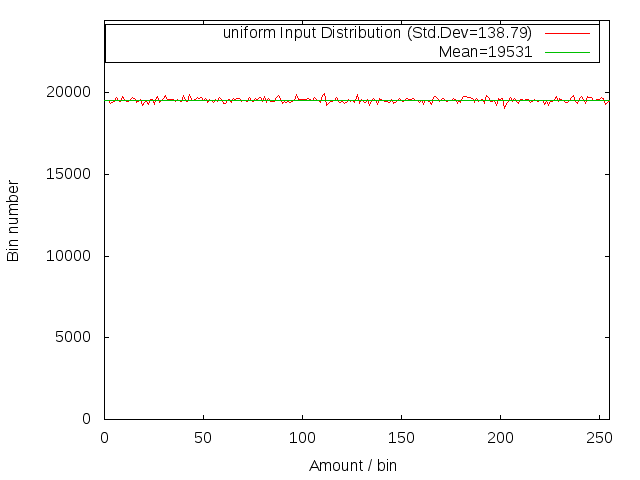
\includegraphics[width=\textwidth]{Graphs/Dist/Tabulation_uniform_dist.png}
    \caption{Uniform Input Distribution}
    \label{fig:tab_dist_uni}
  \end{subfigure}
\end{figure}
\begin{figure}[H]\ContinuedFloat
  \centering
  \begin{subfigure}[b]{0.9\textwidth}
    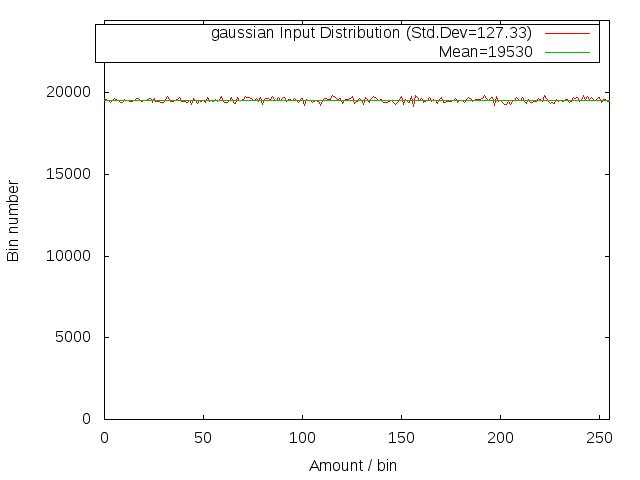
\includegraphics[width=\textwidth]{Graphs/Dist/Tabulation_gaussian_dist.png}
    \caption{Gaussian Input Distribution}
    \label{fig:tab_dist_gauss}
  \end{subfigure}
\end{figure}
\begin{figure}[H]\ContinuedFloat
  \centering
  \begin{subfigure}[b]{0.9\textwidth}
    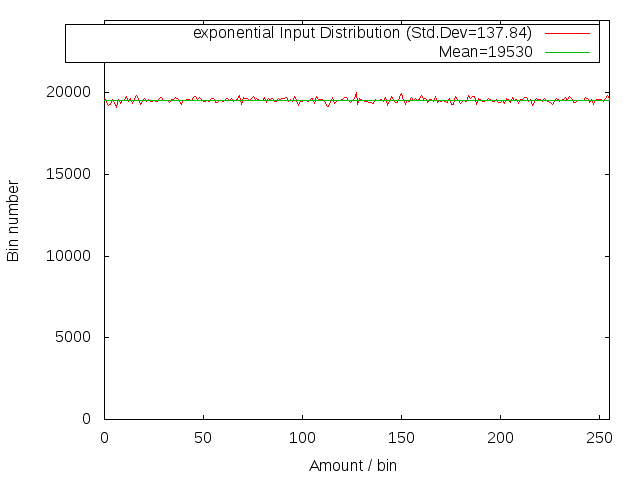
\includegraphics[width=\textwidth]{Graphs/Dist/Tabulation_exponential_dist.png}
    \caption{Exponential Input Distribution}
    \label{fig:tab_dist_exp}
  \end{subfigure}
  \caption{Output Distributions of Tabulation Hashing}\label{fig:tab_dist}
\end{figure}

It can be seen, that for all three input distribution, the output distribution is very close to uniform, thus showing that tabulation hashing will map roughly the same amount of inputs to each hash value. This is also emphasized by the reported standard deviation, which yields a very low coefficient of variance of 0.007. Since the cost of hashing based methods increases drastically as more collisions occurs, a uniform output distribution will yield the best performance. 

\paragraph{Murmur hashing.} Dittrich et al. also found murmur hashing to have shown strong distributional properties, by being very robust. It is therefore also expected that murmur hashing will yield a close to uniform output-distribution for all of the three input-distributions.\\

The output distributions found from the categorized results of running the test using murmur hashing can be seen on the figure \ref{fig:murmur_dist}. 
\begin{figure}[H]
    \centering
    \begin{subfigure}[b]{0.9\textwidth}
        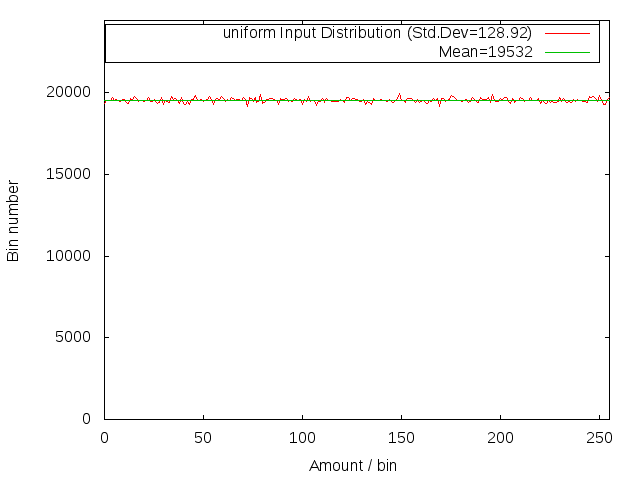
\includegraphics[width=\textwidth]{Graphs/Dist/Murmur_uniform_dist.png}
        \caption{Uniform Input Distribution}
        \label{fig:murmur_dist_uni}
    \end{subfigure}
\end{figure}
\begin{figure}[H]\ContinuedFloat
    \centering
    \begin{subfigure}[b]{0.9\textwidth}
        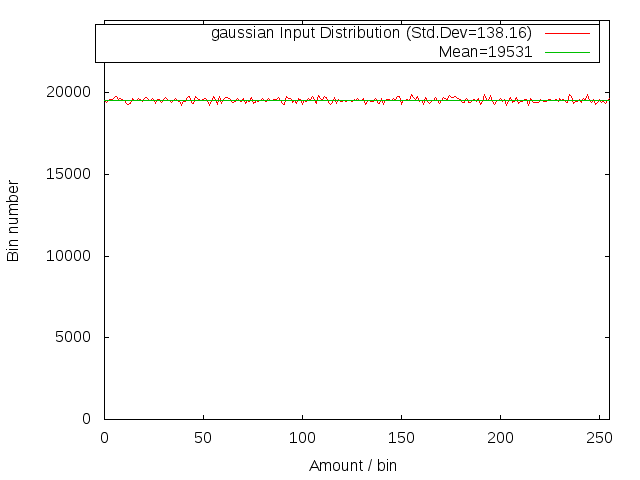
\includegraphics[width=\textwidth]{Graphs/Dist/Murmur_gaussian_dist.png}
        \caption{Gaussian Input Distribution}
        \label{fig:murmur_dist_gauss}
    \end{subfigure}
\end{figure}
\begin{figure}[H]\ContinuedFloat
    \centering
    \begin{subfigure}[b]{0.9\textwidth}
        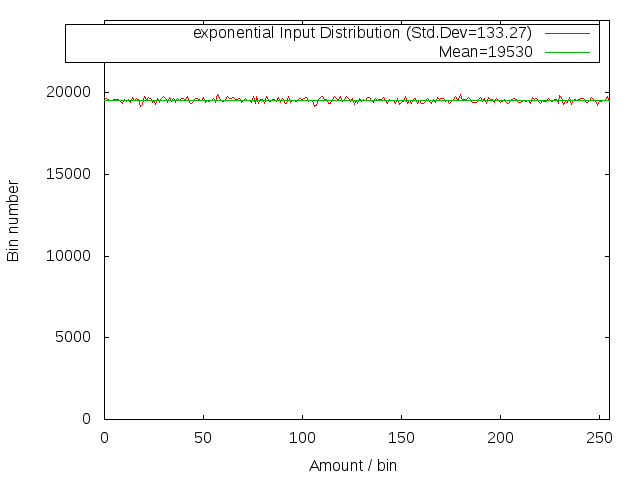
\includegraphics[width=\textwidth]{Graphs/Dist/Murmur_exponential_dist.png}
        \caption{Exponential Input Distribution}
        \label{fig:murmur_dist_exp}
    \end{subfigure}
    \caption{Output Distributions of Murmur Hashing}\label{fig:murmur_dist}
\end{figure}
As seen, the output distributions of murmur hashing appears equally well distributed as the output distributions for tabulation hashing, which also if emphasized by noticing that the standard deviations of the two sets of output distributions are similar.\\

Since both hash functions produce equally good output-distributions, approximately the same amount of collision should occur. Thus, when using these in combination with a given hash index, the results should not affect that one scenario has more collisions than the other. Therefore, any difference in such results would be caused by one hash function having a higher throughput in the given scenario.

\subsubsection{Key-length test}
To have a baseline of how well the two hash functions perform, a single-core evaluation of the performance on various key lengths have been done, by hashing keys of different length and calculating the average runtime of each hashing. This test shows how well the implementation scales over key lengths, when used without any other structures. \\

Since one of the key concepts of tabulation hashing is to utilize rapid lookups in fast cache, we have tried to avoid filling the L1 cache with keys, by choosing to only generate a small amount of strings (i.e. 5) for each of the lengths from 1-64 bytes, yielding 320 strings in total. For each of the 64 string lengths, the 5 strings have been hashed 10.000 times, in order to make the total runtime long enough, for the time-taking to be stable. The duration of the repeated hashings have been measured using \verb|chrono|'s \verb|high_resolution_clock|, yielding the total amount of nanoseconds. 

This entire setup has then been run 10.000 times yielding a total of 100.000.000 hashings of each string, from which an average run-time and a standard deviation can be calculated, for each of the 64 lengths. \\

This experiment is interesting, as it shows an upper bound on how well the two hash functions can perform, but since hash functions rarely are used alone, it does not show the entire picture. For instance, including the tabulation hash with a large index structure might contest the cache more, thus making more cache misses happen and therefore causing a lower throughput. \\

Since tabulation hashing can be specialized for a given maximal key length, by tuning the amount of tables, this would be interesting to include in the test. Therefore, we have run four separate runs for the tabulation hashing function, using 8, 16, 32 and 64 tabulation tables, respectively. It should be noted, that since tabulation hashing cannot hash keys longer than the amount of tabulation tables generated, each of the datasets only run up to the amount of tabulation tables it resembles. Only one run has been done for the murmur hashing function, since it does not contain any tuning parameters. \\

The average run-time for each length can be seen on figure \ref{fig:tab_length}, which contains five data-sets, four for the four tabulation hashing runs using 8, 16, 32 and 64 tabulation tables, respectively, and one for the murmur hashing run. 

\begin{figure}[H]
  \includegraphics[width=\textwidth]{Graphs/Length/4_Tabulation_64_tables_length.png}\\
  \caption{Run-time scalability over different lengths of input string.}\label{fig:tab_length}
\end{figure}
By first looking at the four data-sets for the tabulation hash runs, we see that all of them experiences a similar, close to linear scaling for short key lengths (i.e. up to 16 bytes). They all show the same run-time for hashing strings of just one byte, which takes roughly 6ns, while each additional byte in the string adds roughly 1.5ns. The low cost of the bytes following the first can be explained by that the reads of these bytes can be overlapped with the read of the previous bytes, where reading just the first byte still has to complete an entire read from memory.\\

However, for the two data-sets using 32 and 64 tabulation tables respectively, we see that the scaling becomes less optimal for longer strings. Specifically, both of the two data-sets still show a close to linear scaling for strings longer than 16 bytes, but with a steeper slope of roughly 2-2.5ns per additional byte. 

This can be explained by looking what the additional bits causes to happen in the implementation. Since each byte causes a lookup in its own table, using longer strings will cause lookups in more tables. This will in turn cause more cache-lines to be loaded into the cache, which leads to more contention and therefore more cache misses. The overhead caused by this is however quite small, which indicates that most of the data must be resident in the next level of cache (i.e. L2).\\

Secondly, it should be noted that while the four data-sets for tabulation hashing all appear close to linear, the standard-deviation (seen on the error bars) increases, as the amount of tables is increased, as well as when the length of the strings are increased. This is most likely caused by the same contention as before.\\

\textcolor{red}{Finish this conclusion with data from napoleon}
Finally, it can easily be seen that while the tabulation hashing has a slightly better performance on very short strings (i.e. up to 3 bytes), the murmur hashing function scales better on the length of the key, since every 4 additional bytes in the key only increases the run-time of each hash by roughly 2ns. The murmur hashing takes ~10ns to hash a key of length 1 byte, and spends the same amount of time hashing strings of length up to 4 bytes. \\

Additionally, the increase in run-time only appears to happen after every fourth additional byte. This is caused by that the body-loop of the murmur hashing implementation, which is where the additional length of the key is handled, is iterated once for every 32-bit chunk of the key. It can thus be concluded that the increase in run-time primarily comes from additional iterations of this loop, while the difference in 0-3 bytes in the tail does not affect much.

\subsubsection{Multi-core test}
To test the scalability across multiple cores, we have created test-setup similar to the key-length test, run it on multiple threads, and measured the throughput of each thread as well as the total throughput. This was done by initializing one hash function object~\footnote{Either of class \verb|tabulation_hash| or of class \verb|murmur_hash|}, which is used by all the threads in their computations. The threads are all pinned to a specific core, to avoid reduced performance, e.g. from potentially having more cache misses. Each thread is given its own set of 5 strings, to avoid sharing of this memory region, which is then hashed 100.000.000 times, from which an average total throughput can be calculated. \\

Since neither of the hash function classes contain any shared state which is modified after initialization, a perfect linear increase in throughput would be expected, when more cores are being utilized.\\

On Figure \ref{fig:tab_cores} the average total throughput is shown for both tabulation hashing and murmur hashing. As in the key-length test, we have included four data-sets for the tabulation hashing, using 8, 16, 32 and 64 tabulation tables, respectively. Since the purpose of this graph is showing how well each of the configurations scale, rather than evaluating the throughput using a given core, the length of the keys has been fixed to be the highest amount possible, which is therefore equal to the amount of tabulation tables for the tabulation hash sets, and 64 for the murmur hash set. 

Additionally, a linear function with slope equal to the throughput found when using just one thread has been added for each of the data-sets, which show the perfect throughput scaling.\\

\begin{figure}[H]
  \includegraphics[width=\textwidth]{Graphs/Cores/4_Tabulation_8_tables_cores.png}\\
  \caption{Throughput using different amounts of threads.}\label{fig:tab_cores}
\end{figure}
While it from this graph might appear that tabulation hashing with 8 tabulation tables has best overall performance, do remember that it has been hashing key of length 8, while all the other data-sets are generated by hashing longer keys. This also means that while tabulation hashing with 16 tabulation tables and murmur hashing seems to have the same throughput, but the former hashes keys of length 16, while the latter hashes keys of length 64. However, since the yield of the graph is an understanding of the scalability of the setups, the data-sets should not be compared to each other.\\

First note that all of the data-sets show three different linear sections (most apparent on the red curve), with different slopes. The first section shows very close to perfect scaling up to 8 cores. In the next section (9-16 cores), the increase appears linear but with a reduced slope, thus indicating less optimal scaling. Finally, after 16 cores the scaling is reduced even further. \\

To understand this behavior, we will refer to the scalability-behavior described in the hardware setup~\ref{subsec:hardware} on page~\pageref{subsec:hardware}. This scalability behavior very much resembles the behavior found with the dummy-workload, which might indicate that the found scalability behavior of the hash functions is caused by the factors described there. \\

Since we have seen this exact behavior for different amounts of work of the dummy-workload, it would appear that the reduction in scalability is a percentage of the total throughput, instead of an absolute overhead. As such, a similar percentage wise reduction in performance is to be expected for these test cases. \\

However, since we have no way of verifying that this is the sole cause of the reduced scaling, the primary take-away from the graph is the close to perfect scalability of all five data sets for the first 8 cores. Whether or not the baseline scalability properties of the setup accounts for the entire reduction of throughput after 8 cores cannot be determined, while the reduction itself neither can be used to conclude that the hash functions does not scale properly.

\subsection{Experiments on hashing indices}
As previously stated, the YCSB framework provides an apples-to-apples comparison, by fixing standardizing the foundation of the comparison. Throughout the following paragraphs, our implementation will be described, and in the next subsection, the primary differences to the traditional YCSB framework will be described and discussed.\\

One of the primary components to be standardized is the generation of data to be loaded into the database, as well as the generation of operations making up the workloads to be performed. Another key component is the \verb|workload_properties|, which define the work to be performed, independent of any database specific information. These standardizations are handled by the \verb|workload| class, which has methods for generation of data and operations to be performed, based on a set of \verb|workload_properties|. This is to be seen as a replacement for the default \verb|CoreWorkload| implementation of the workload executor of the YCSB framework.\\

The other key class of the YCSB framework is the \verb|client| class, which spawn the wanted amount of threads and instantiates a \verb|workload| for each of the threads to use. The threads each perform a sequential series of operations, in order to either load or perform transactions on the database system, which the generate using their \verb|workload|. The loading and transactions are done by invoking the \verb|workload| class to interact with the database interface, \verb|abstract_index|, which yields functions representing the standard CRUD operations, namely 'create', 'read', 'update' and 'delete'. Since range scans are included, the 'read' operation is split into single-key reads (in the \verb|read| function) and multi-key reads (in the \verb|range_scan| and \verb|reverse_rande_scan| functions). \\

A class diagram for these two classes can be seen on Figure~\ref{fig:UML_YCSB}. As seen, the \verb|client| is instantiated with a database implementation (anything that adheres to the \verb|abstract_index| interface), as well as a set of \verb|workload_properties|, which defines the workload to be executed. It then instantiates an instance of the \verb|workload| class for each thread, which is used for generating the data and operations for the thread to perform. \\

The \verb|workload_properties| struct defines the workload to be executed, which thus controls the parameters to be standardized, such as read/write-proportions, key and value maximum lengths and which distributions to use for generating the data. The six core workloads are simply specific instantiations of this struct, which makes extending the core workloads extremely easy. \\

The \verb|client| class has been implemented in the \verb=client.[h|cc]= files\footnote{For interfaces of the \verb|client| and the \verb|workload| class, refer to the class diagrams on Figure~\ref{fig:UML_YCSB}}. It allows a given workload to be run against the given database system through calling the \verb|run_workload| function with a wanted amount of threads. It spawns the given number of threads, which first load the database system and then perform transactions. The threads each monitor the duration of the transaction-phase, and calculates the throughput performed. These durations are yielded to the \verb|run_workload| function, which calculates and returns the total throughput of all threads, over the transaction part. For the possibility of increased control, this has also been split into two different functions, namely \verb|run_build_records| and \verb|run_transactions|, which handles the loading and transaction parts, respectively. \\

The workload executor class, \verb|workload|, has been implemented in the \verb=workload.[h|cc]= files. The two main functions exposed are the \verb|do_insert| and \verb|do_transaction| function, which both take an \verb|abstract_index| as parameter, performs an insertion or transaction into the database, respectively. Besides these two functions, only the two functions \verb|get_record_count| and \verb|get_operation_count|, which yield the amount of loading operations and transaction operations to be performed, respectively. Therefore, the following will focus on the implementation of the two former functions.\\

The two main functions are quite similar, as they both generate the content for a given single operation, and perform it. While \verb|do_insert| always performs an insertion operation on the database, in order to load it, \verb|do_transaction| first generates an operation to perform, based on the operation-distribution defined in the \verb|workload_properties|. \\

The generation of keys also differ for the two phases. For the loading phase, a simple counter generator is used, which ensures unique keys by incrementing an internal counter. For the transaction phase, the \verb|workload_properties| define a distribution, with which a key from set of inserted keys is drawn. This distribution is either uniform, zipfian, or latest\footnote{Their own zipfian distribution, which yields the highest weight on the last drawn value}. \\

For the operations which require a value (i.e. insert, update, read-modify-write), a value is generated, by first uniformly selecting a value length up to a maximum defined in the \verb|workload_properties|, and then adding a random byte to an empty string until the given length is reached.\\

Finally, when the operation, key and (potentially) value has been generated, the \verb|workload| invokes the appropriate function on the database.\\
\paragraph{Key differences from traditional YCSB.} As mentioned, there are a couple of differenced between the implementation, and the YCSB framework as it was developed by B. Cooper. First of all, since the focus of this project has been the scalability of the multi-core in-memory key-value stores, we have chosen to omit tracking of latency for individual operations. As part of the latency test, the original YCSB framework enables threads to throttle the throughput, in order to test how good the latency is under certain load pressures. This has therefore also been omitted. \\

Secondly, the original implementation is targeted on database systems, in which a record can hold multiple fields. Our implementations of key-value stores only allow single-field values, and as such this would have to be omitted as well. However, since more fields implies more load pressure on the system, since more data has to be loaded/stored, we have enabled values to have variable length. This simulates having a different amount of fields, and is only limited by the fact that you have to operate on all the fields at once, where the original implementation allows operations of subsets of the fields.\\

Lastly, to completely avoid any sharing of memory regions between threads, we have chosen to instantiate a \verb|workload| class for each of the threads, where the original implementation only uses one. The throughput each thread produces is measured in operations, which thus include the generation of keys and values. Since the \verb|workload| class is responsible for all the generation, it uses random generators. If we were to use the same \verb|workload| for all threads, they would be sharing the state of the random generators, causing a potential source of contention, which is not intended. Using one \verb|workload| for each does completely avoid any shared state, thus eliminating a source of contention.\\

\begin{figure}[H]
  \makebox[\textwidth][c]{\includegraphics[width=1.15\textwidth]{UML/YCSB.png}}\\
  \caption{Class diagram for the YCSB framework implementation.}\label{fig:UML_YCSB}
\end{figure}
\paragraph{Tuning of experiments.}
We have chosen to only use the core-workloads of the YCSB framework, and thus not use the extensibility of the framework to create new workloads. This was chosen, as we have found the core-workloads to yield a proper comparison-foundation, while we did not find much value in tuning the \verb|workload_properties|. Instead, we have identified the primary tuning parameters in the hashing schemes and performed experiments with these, to find an understanding of the trade-offs connected to this tuning. This will be presented first, as the results will yield a proper set of hashing scheme parameters to perform the YCSB core workloads with.\\
\\
The primary tuning parameters are,
\begin{itemize}
  \item Maximal key length (tabulation tables), for tabulation hashing
  \item Directory size, for array hashing
  \item Initial global depth, for extendible hashing
  \item Prefix bits (amount of partition), for partitioned array hashing
\end{itemize}
\subparagraph{Maximal key length (Tabulation Hashing).} The maximal key length is a bit different from the remaining three parameters, in that it does not present a trade-off between operation throughput and memory consumption. Rather, as we have seen previously, using less tabulation tables causes less cache-lines to be loaded, and therefore less contention on the L1 cache. This causes a performance gain. The downside of fewer tabulation tables is obviously that the maximum length on the keys will be reduced. This parameter will therefore have to be set based on an evaluation of the specific use case, determining if longer keys will be present or not.\\

The three remaining tuning parameters all yield a trade-off between performance and memory usage. 
\subparagraph{Directory size (Array Hashing).} For the directory size of array hashing, inserting the same amount of keys into a larger directory means less entries in each bucket, as there will be more buckets to distribute between. Since all the operations traverse the bucket for a given key, this means shorter run-times for all of the operations, thus yielding an overall higher throughput. However, as each bucket has a memory overhead from the additional pointer to the bucket, as well as the vectors' \verb|begin|, \verb|end| and end-of-capacity pointers and its allocator, more buckets will cause more memory to be used. The memory overhead for each bucket is 36B, as we have 7 pointers + two allocators~\footnote{1 pointer to the bucket, and two vectors (keys and values), each having 3 pointers and an allocator}. Since both the key and the value of a single entry are strings, one entry could quickly amount up to as much memory. Thus, as long as the majority of the buckets are not empty once the database has been loaded up to an expected load, the memory overhead of the additional buckets will be outweighed by the memory used by the actual data stored.\\

To verify this, an experiment has been conducted, in which the directory size has been varied for values between $2^4$ and $2^{20}$. Since the change in performance is caused by the lower probing time, we have chosen to run this experiment over the c-core-workload, as this includes 100\% read-operations, which are expected to have lowest run times. The throughput as well as the peak memory usage for different directory sizes can be seen on Figure~\ref{fig:dir_size}.

\begin{figure}[H]
  \centering
  \includegraphics[width=0.9\textwidth]{Graphs/dir_size.png}\\
  \caption{Throughput and memory usage for various directory sizes of array hashing.}\label{fig:dir_size}
\end{figure}

\subparagraph{Initial global depth (Extendible Hashing).} The initial global depth of extendible hashing is quite similar to the directory size of array hashing, while it has some key difference. First of all, the global depth defined is only valid initially, as this can increase. As such, poor choice of this tuning parameter will eventually solved by the algorithm itself. Secondly, since the buckets has a fixed size in extendible hashing, there is a fixed upper limit on the probing time. There will therefore never be much contention in any buckets, which means that performance gain on the probing times will be less significant.\\

The key advantage of choosing a proper value for the initial global depth comes from avoiding the 'slow path' of the insert algorithm, as a larger initial global depth makes splits of the directory less frequent. Since the 'slow path' requires exclusive access to the entire directory (and thus the entire data structure), reducing the amount of runs through this path will yield an increase in the insertion throughput. \\

This performance increase will be quite insignificant over the course of many operations. A simple calculation can yield an upper limit on how many times the 'slow path' can be taken. Each run through the slow path causes at least a doubling of the directory, and therefore every such run will double the memory overhead from the bucket pointers. Thus, just 30 runs through the 'slow path' will cause a minimal initial directory of 1 bucket to have a memory overhead from bucket pointers of 4.29GB, which is doubled by every following run, completely ignoring the memory used by the actual data. This will quickly hit a memory capacity of the machine, thus ensuring that a low amount of runs through the 'slow path' will happen in any setup.\\
\\

A secondary performance increase of the insert operation comes from the fact that a bucket is instantiated for every entry in the preallocated directory. Thus, a higher initial global depth causes more buckets to be instantiated initially, which will not have to be instantiated during the execution of actual work. \\

This does however also mean that the memory overhead of an increased preallocation of the directory for extendible hashing is just as large as for array hashing. While a doubling of the directory as part of a insertion operation only creates new pointers to the original buckets, and therefore has a much lower memory overhead than the additional buckets created for a larger directory size in array hashing, the amount of bucket initially generated is equal to the size of the directory, and thus directly linked to the initial global depth. \\

Totally, we can see that the extendible hashing algorithm is more robust to a poor preallocation, has a less significant performance gain of a proper tuning of this parameter, and has an equally large memory overhead from a large preallocation.
\textcolor{red}{The experiment performed is based on the transaction phase, thus the issue will most likely be fixed in the loading phase}
\subparagraph{Prefix bits (Partitioned Array Hashing).} 
For the partitioned array hashing, the primary 

\newpage
\textcolor{red}{paragraph about heterogeneous tuning}
\section{Discussion}
\newpage
\section{Conclusion}
\newpage



\begin{thebibliography}{99}

\bibitem{Zobrist}
 Zobrist, A.\\
 \emph{A New Hasahing Method with Application for Game Playing.}\\
 http://research.cs.wisc.edu/techreports/1970/TR88.pdf

\bibitem{WC79}
 Carter, J.; Wegman, Mark.\\
 \emph{Universal classes of hash functions.}\\
 Journal of Computer and System Sciences, 143-154:\\
 https://www.cs.princeton.edu/courses/archive/fall09/cos521/Handouts/universalclasses.pdf

\bibitem{TZ09}
 Thorup, M.; Zhang, Y.\\
 \emph{Tabulation based 5-universal hashing and linear probing.}\\
 In Proc. 12th Workshop on Algorithm Engineering and Experiments (ALENEX), 2009

\bibitem{PT11}
 Pătraşcu, M.; Thorup, M.\\
 \emph{The Power of Simple Tabulation Hashing}\\
 http://arxiv.org/abs/1011.5200

\bibitem{RAD15} % 0
 Ritcher, S.; Alvarez, V.; Dittrich, J.\\
 \emph{A seven Dimensional Analysis of Hashing Methods and its Implications on Query Processing}\\
 http://www.vldb.org/pvldb/vol9/p96-richter.pdf

% Hash Tables
\bibitem{ItA09}
 Cormen, Thomas H.; Leiserson, Charles E.; Rivest, Ronald L.; Stein, Clifford (2009). \\
 \emph{Introduction to Algorithms (3rd ed.).} \\
 Massachusetts Institute of Technology. pp. 253–280. ISBN 978-0-262-03384-8.

\bibitem{NA09} % 1
 Askitis, N.\\
 \emph{Fast and Compact Hash Tables for Integer Keys}\\
 http://dl.acm.org/citation.cfm?id=1862675

\bibitem{AJ05}
 Askitis, N.; Zobel, J.\\
 \emph{Cache-Conscious Resolution in String Hash Tables}
 http://goanna.cs.rmit.edu.au/~jz/fulltext/spire05.pdf

\bibitem{ADSJ13} % 6
 Dudás, Á.; Juhasz, S.\\
 \emph{Blocking and non-blocking concurrent hash tables in multi-core systems}\\
 http://www.wseas.org/multimedia/journals/computers/2013/5705-125.pdf

\bibitem{BC10}
 Cooper, B. F.; Silberstein, A.; Tam, E.; Ramakrishnan, R.; Sears, R.\\
 \emph{Benchmarking Cloud Serving Systems with YCSB}\\
 https://www.cs.duke.edu/courses/fall13/cps296.4/838-CloudPapers/ycsb.pdf

\bibitem{Mur3}
 Appleby, A.\\
 \emph{Original Murmurhash3 implementation}\\
 https://github.com/aappleby/smhasher, version 08/01/16

\bibitem{DPH90}
 Dietzfelbinger, Martin, et al. \\
 \emph{Dynamic perfect hashing: Upper and lower bounds.}
 SIAM Journal on Computing 23.4 (1994): 738-761.

\bibitem{nphf}
 \emph{Napoleon machine, for the HIPERFIT research center}\\
 http://napoleon.hiperfit.dk/

 

\end{thebibliography}
\end{document}
